% =============================================================================
%  Dinamica3_Fase3_Diapositiva2.tex — Dinámica 3, Fase 3, Diapositiva 2:
%  la falla del filtro. Bokeh agresivo (luces grandes, saturadas y opacas
%  sobre el texto) y desenfoque severo de todo el bloque: ya no hay capa nítida.
%  Formato 16:9. Compilar con: bash ../../../compilar_diapositivas.sh
% =============================================================================
\documentclass[tikz,border=0pt]{standalone}
\usepackage[utf8]{inputenc}
\usepackage[T1]{fontenc}
\usepackage{ebgaramond}
\usetikzlibrary{fadings}
\frenchspacing
\hyphenpenalty=10000 \exhyphenpenalty=10000   % sin división de palabras

% ── Parámetros ────────────────────────────────────────────────────────────────
%  \Difuminado: intensidad del desenfoque (0 = nítido, 1 = ilegible).
%  Fase 3: desenfoque severo, rango sugerido 0.70 – 0.85.
\def\Difuminado{0.75}
\def\RadioMax{6}        % radio máximo del desenfoque, en pt (con \Difuminado = 1)
\def\TamLetra{30}       % tamaño de letra, en pt
\def\Interlinea{42}     % interlineado, en pt
\def\AnchoTexto{25}     % ancho del bloque de texto, en cm
\def\NumLuces{70}       % luces del bokeh agresivo

% ── Paleta ────────────────────────────────────────────────────────────────────
\definecolor{Pergamino}{HTML}{E9DCC2}
\definecolor{PergaminoTension}{HTML}{A98652}
\definecolor{Tinta}{HTML}{2B2620}
\definecolor{Referencia}{HTML}{3E3122}
\definecolor{LuzNaranja}{HTML}{FF6B1A}
\definecolor{LuzMagenta}{HTML}{E8368F}
\definecolor{LuzCian}{HTML}{22B8CF}
\definecolor{LuzAmarilla}{HTML}{FFD23F}
\definecolor{LuzBlanca}{HTML}{FFFFFF}

% ── Dimensiones (16:9) ────────────────────────────────────────────────────────
\def\ancho{32}
\def\alto{18}

\newcommand{\Bloque}{%
  \textbf{La novela:} un hombre deja sus negocios en
  Jerez tras la muerte de su padre y se muda a Madrid; su tío quiere
  hospedarlo, pero él cuida su independencia.\par\vspace{0.8em}
  \textbf{Oliveira:} se pregunta cómo alguien puede
  engancharse a una novela mal escrita y a revistas triviales, y admite
  que, tras unas páginas, uno ya no puede dejar de leer.%
}

\begin{document}
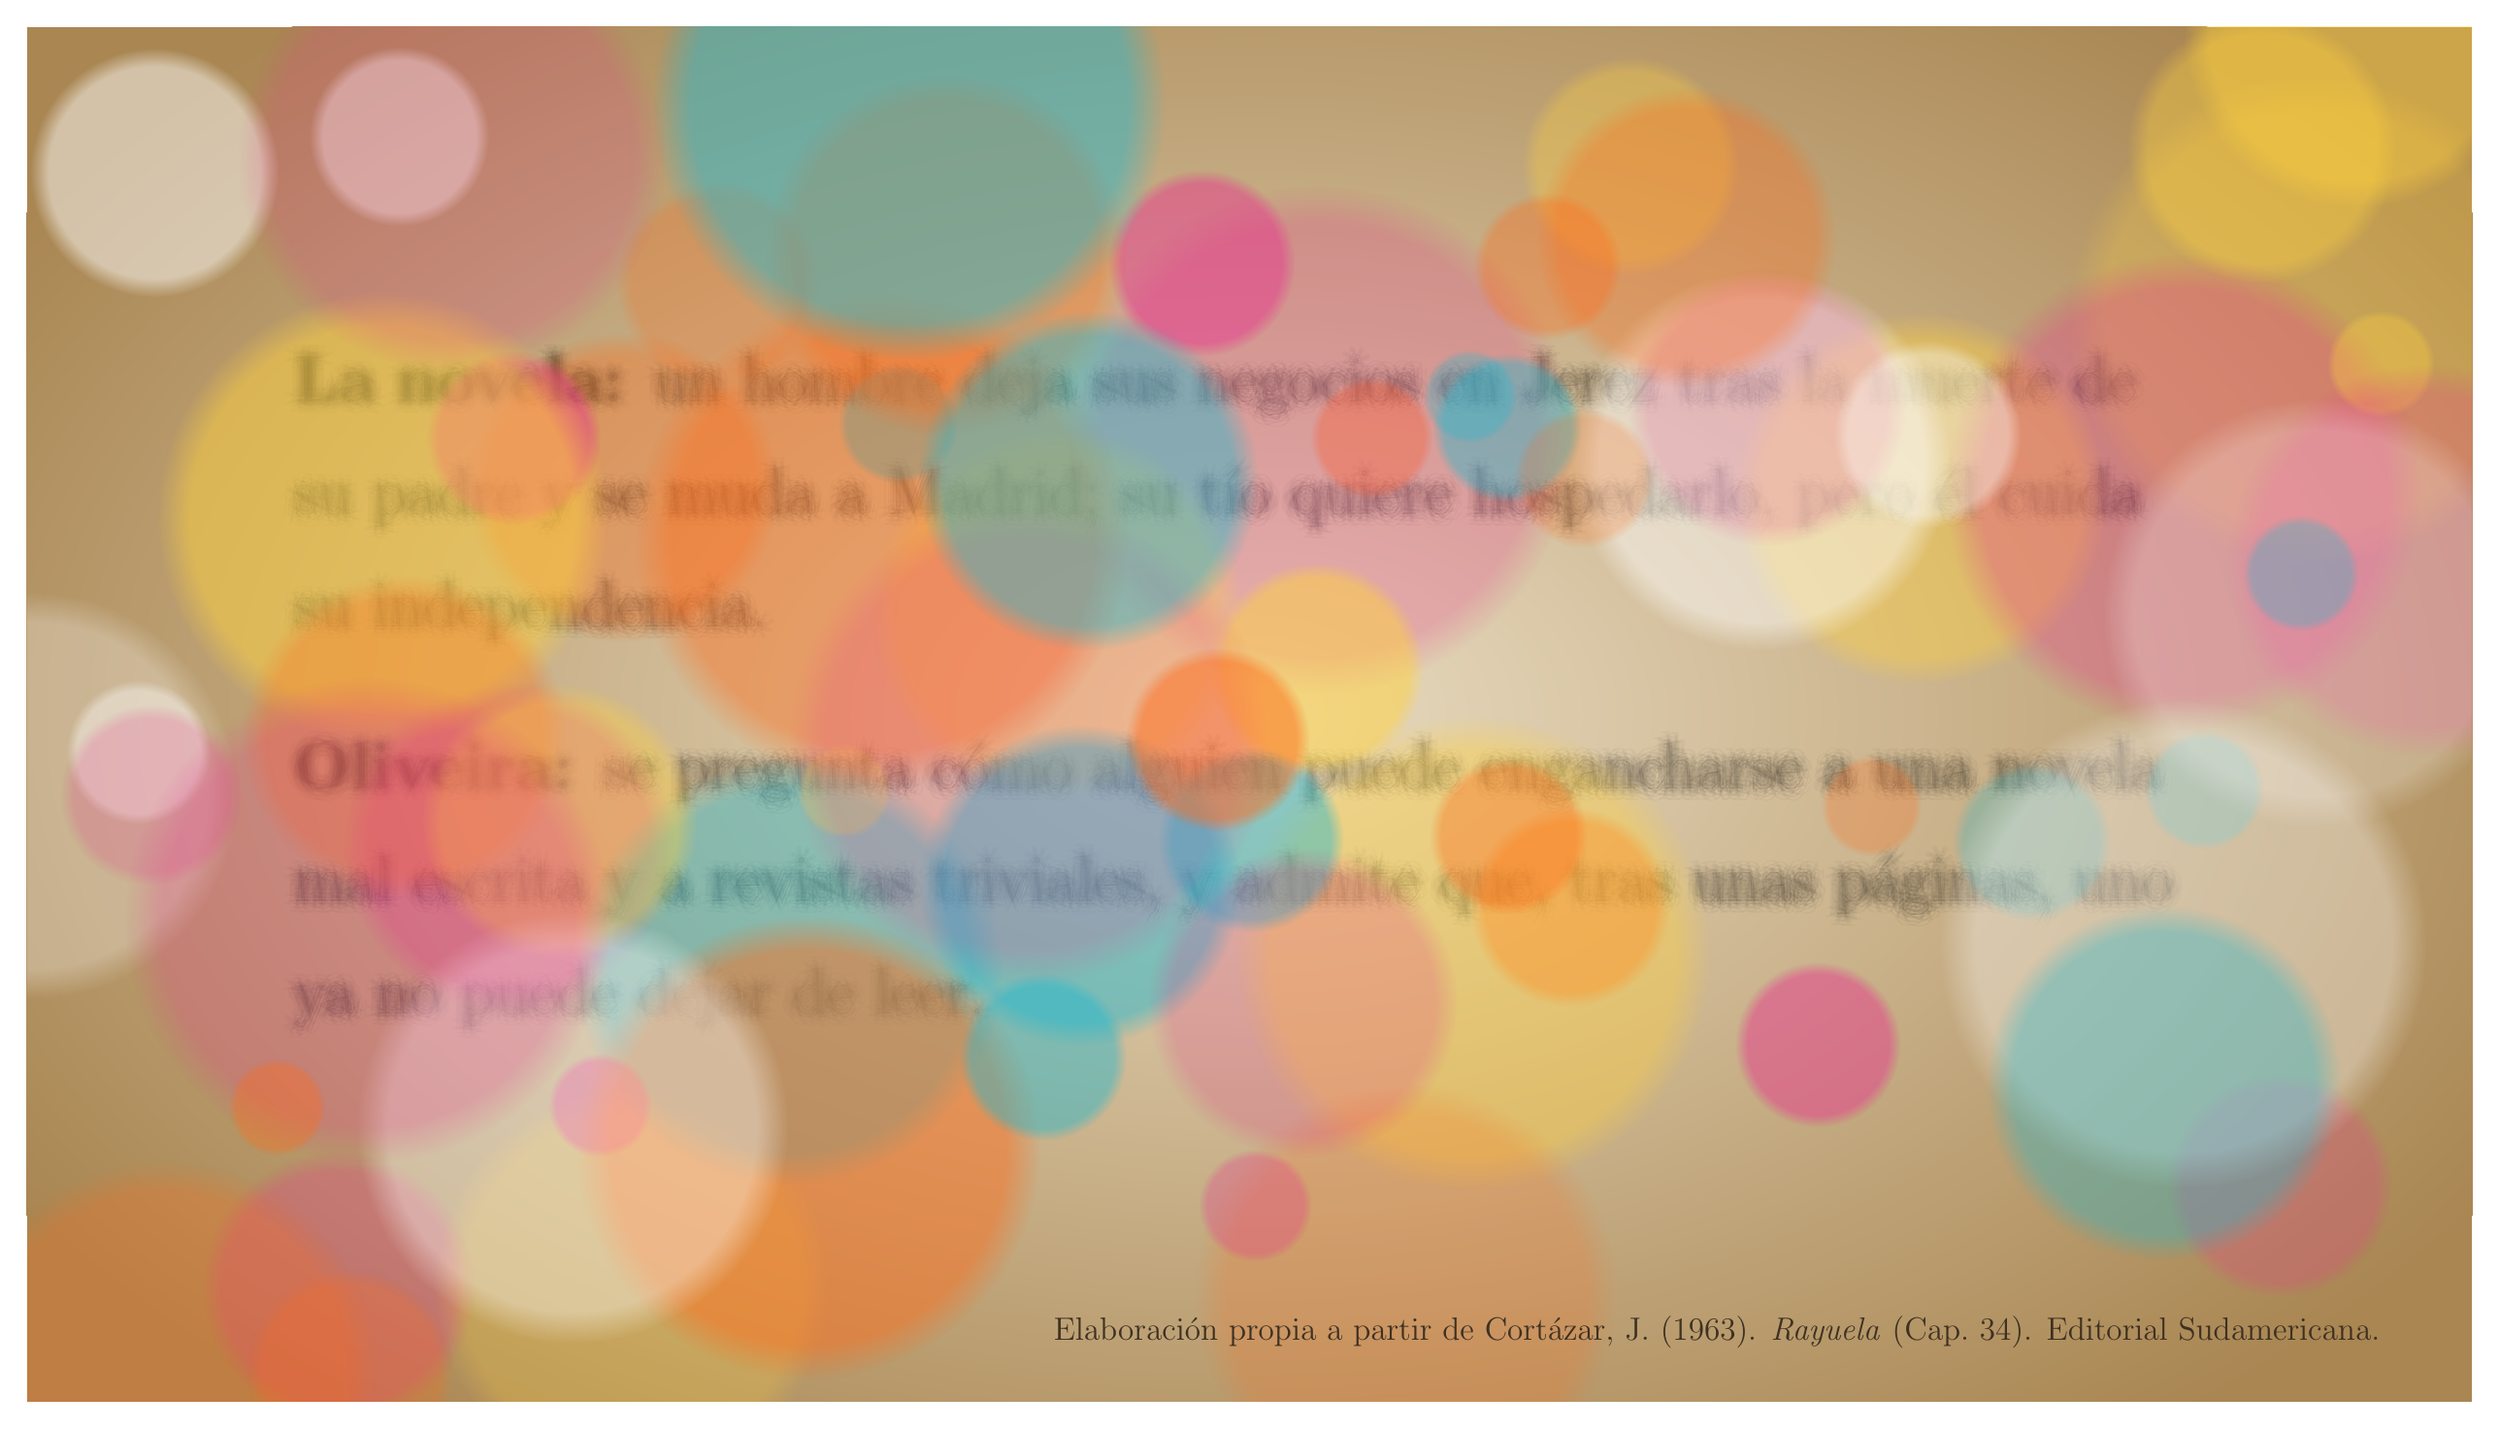
\begin{tikzpicture}
  \useasboundingbox (0,0) rectangle (\ancho,\alto);
  \clip (0,0) rectangle (\ancho,\alto);

  % Fondo: pergamino oscurecido, viñeta intensa
  \fill[PergaminoTension] (0,0) rectangle (\ancho,\alto);
  \shade[inner color=Pergamino, outer color=PergaminoTension]
    (\ancho/2,\alto/2) ellipse [x radius=0.60*\ancho, y radius=0.66*\alto];

  % Texto con desenfoque severo: tres anillos de copias, sin capa nítida
  \tikzset{bloque/.style={anchor=center, align=left, inner sep=0pt,
    text width=\AnchoTexto cm, font=\fontsize{\TamLetra}{\Interlinea}\selectfont}}
  \coordinate (centro) at (\ancho/2,\alto/2+0.3);
  \pgfmathsetmacro{\R}{\Difuminado*\RadioMax}
  \foreach \ang in {0,45,...,315}{
    \foreach \f/\op in {1/0.04, 0.66/0.05, 0.33/0.06}{
      \node[bloque, text=Tinta, text opacity=\op]
        at ([shift={(\ang+15*\f:\f*\R pt)}]centro) {\Bloque};
    }
  }
  \node[bloque, text=Tinta, text opacity={0.6*(1-\Difuminado)}]
    at (centro) {\Bloque};

  % Bokeh agresivo encima del texto (semilla fija)
  \pgfmathsetseed{1968}
  \foreach \i in {1,...,\NumLuces}{
    \pgfmathsetmacro{\x}{rnd*\ancho}
    \pgfmathsetmacro{\y}{rnd*\alto}
    \pgfmathsetmacro{\r}{0.6+2.9*rnd^1.5}
    \pgfmathsetmacro{\o}{0.18+0.32*rnd}
    \pgfmathtruncatemacro{\c}{int(5*rnd)}
    \ifcase\c\relax \def\col{LuzNaranja}\or \def\col{LuzMagenta}%
      \or \def\col{LuzCian}\or \def\col{LuzAmarilla}\else \def\col{LuzBlanca}\fi
    \fill[\col, fill opacity=\o, path fading=circle with fuzzy edge 15 percent]
      (\x,\y) circle (\r);
  }

  % Referencia
  \node[anchor=south east, text=Referencia, inner sep=0pt,
        font=\fontsize{13}{16}\selectfont]
    at (\ancho-1.2,0.7)
    {Elaboración propia a partir de Cortázar, J. (1963). \textit{Rayuela} (Cap.~34). Editorial Sudamericana.};
\end{tikzpicture}
\end{document}
